% !TEX spellcheck = en_US
%=================================================================================
\chapter{Controller design objectives}
%=================================================================================
\section{Advanced Controller}

Wind turbine use closed-loop control (maximum energy capture over normal operation and less structural load) systems to continuously adjust their operations based on feedback. Figure 1, illustrates the advanced closed-loop control diagram of a wind turbine. 
\\[16pt]
The torque controller optimizes power production below rated speed and maintain rated power above rated wind speed by adjusting generator torque $(M_G)$ based on generator speed $(\Omega_G)$. Advance torque control uses a PI controller with anti-windup to regulate the generator torque based on the difference between the actual and reference generator speeds. Above rated wind speed, Pitch controller maintains the rated generator speed $(\Omega_{G,rated})$ by adjusting blade pitch angle $(\theta)$, which ensures the rated power is maintained. With increasing wind speed, the pitch angle increases to reduce power coefficient $(c_p)$. Once the wind speed reaches the rated value, the generator torque is maintained at its rated value. The control is categorized into different regions, as detailed in Section 2.2.

\begin{figure}[htbp]
	\centering
	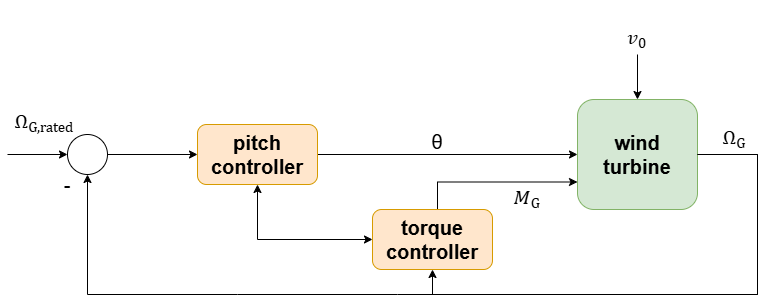
\includegraphics[width=\textwidth]{Figure/Figure_1.png}
	\caption{Advance Wind Turbine Controller}
\end{figure}
 

\section{Control Region}

Wind turbine operations are segmented into three primary regions based on varying wind speed. These regions are defined by the turbine power output relative to wind speed. These regions are detailed below and illustrated in Figure 2.

\begin{figure}[htbp]
	\centering
	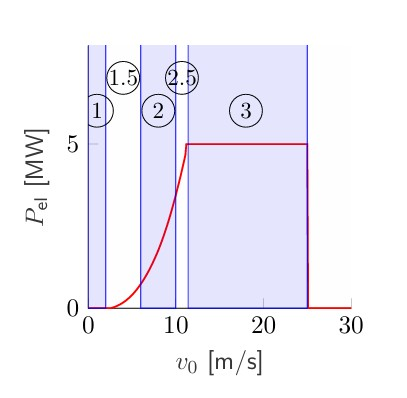
\includegraphics[width=0.5\textwidth]{Figure/Figure_2.jpg}
	\caption{Wind turbine control regions}
\end{figure}

\textbf{Region 1:} When the wind speed is below the cut-in speed $(v_{in})$, the turbine does not generate any power and remains stationary.
\\[16pt]
\textbf{Region 1.5:} This phase indicates the shift to Region2, where wind speeds are sufficient to accelerate rotor. The generator torque is Carefully controlled to accelerate the transition to Region 2. While energy production has started, the power output remains relatively low. The goal is to quickly reach Region 2, where the turbine can operate more efficiently. 
\\[16pt]
\textbf{Region 2:} Wind speeds are above the cut-in speed $(v_{in})$ but below the rated wind speed $(v_{rated})$. The primary objective is to maximize energy yield. To achieve this, the turbine operator at the optimal power coefficient $(c_{P,opt})$, which is determined by reaching the optimal tip seed ratio $(\lambda_{opt})$ and pitch angle $(\theta_{opt})$. The control system ensures that the turbine maintains these optimal conditions by regulating the rotational speed through the torque controller. In this region, the generator torque is adjusted based on rotor speed, as shown in Equation 2.1.

\begin{equation}
	M_{G} = \frac{1}{2} \rho R^5 \frac{P,opt}{{\lambda_{opt}^3 r_{GB}^3}} \Omega_{G}^2
\end{equation}

\begin{equation}
	M_{G} = k\Omega_{G}^2
\end{equation}

\textbf{Region 2.5:} This phase represents a transition between Region 2 and Region 3. In this region, the wind speed is increasing, and the turbine is approaching its rated wind speed. The control system continues to optimize the generator torque to ensure a smooth transition. Energy production is higher compared to Region 2, but the turbine has not yet reached its maximum power output. The pitch controller begins to act to keep the thrust on the rotor as low as possible while aiming to reach the rated speed as quickly as possible.


\textbf{Region 3:} In this region, wind speeds have reached the rated wind speed, and the primary goal is to generate maximum power. The control goal is maintain rated power and generator speed as well as reduce structure loads. The torque controller maintains the generator torque at its rated value. The pitch controller actively adjusts the blade pitch angle to regulate the power and keep it within the turbine rated capacity.

\section{Advanced Generator Torque controller}
Generator torque is one of the two main control inputs for a wind turbine. The performance of an advanced generator torque controller offers significant improvements and greater flexibility compared to a baseline torque controller. The primary goals of the advanced torque controller are to reach the optimal power curve earlier and to maintain it for a longer duration compared to the baseline controller. Additionally, the dynamics in Regions 1.5 and 2.5 are tunable, allowing for more precise control.
\\[16pt]
Goals of the advanced torque controller:

\begin{itemize}
	\item Achieve the optimal power curve earlier.
	\item Maintain the optimal power curve for a longer period.
	\item Enable tunable dynamics in Regions 1.5 and 2.5.
\end{itemize}

\begin{figure}[htbp]
	\centering
	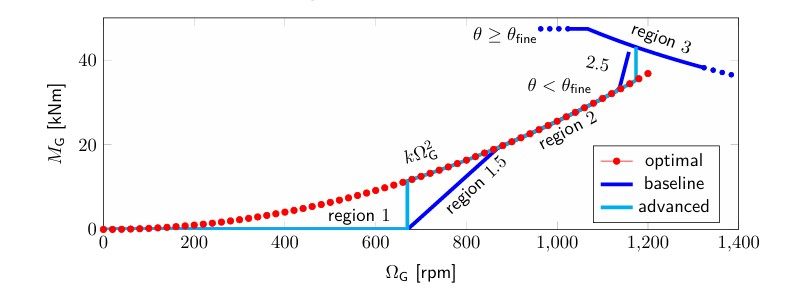
\includegraphics[width=\textwidth]{Figure/Figure_3.jpg}
	\caption{Wind turbine control regions}
\end{figure}

Strategy for the Advanced Torque Controller:

\textbf{Region 1.5:} Lowest generator speed $\Omega_{G,1.5}$ to avoid the 3P frequency interacting with the tower's eigenfrequency. Torque PI controller used for fine-tuning.

\textbf{Region 2.5:} Generator speed $\Omega_{G,2.5}$ = $\Omega_{G,rated}$.
Switch from $\Omega_{G,1.5}$ to $\Omega_{G,2.5}$ if the measured generator speed $\Omega_{G}$ exceeds 

\begin{equation}
	\Omega_{G,R2switch} = \frac{1}{2} (\Omega_{G,1.5} + \Omega_{G,2.5})
\end{equation}

Torque Limits: 

The generator torque limits are determined by the measured generator speed $\Omega_{G}$ and incorporate Anti-Windup mechanisms.

\begin{itemize}
	
	\item if $\Omega_{G}$ < $\Omega_{G,R2switch}$:
	
	\begin{equation}
		M_{G,lb} = 0
	\end{equation}
	\begin{equation}
		M_{G,ub} = k \Omega_{G}^2
	\end{equation}
	
	\item if $\Omega_{G}$ > $\Omega_{G,R2switch}$:
	
	\begin{equation}
		M_{G,lb} = k \Omega_{G}^2
	\end{equation}
	\begin{equation} M_{G,\text{ub}} = \min\left(M_{G,\text{rated}} \frac{\Omega_{G,\text{rated}}}{\Omega_{G}}, M_{G,\text{max}}\right) \end{equation}
	
\end{itemize}


\textbf{Region 2:} The controller aims to maximize energy yield while ensuring the turbine operates efficiently.

\textbf{Region 3:} The torque controller maintains the generator torque at the rated value to protect the turbine from excessive mechanical stress due to high wind speeds.

\section{Collective pitch controller CPC Julius}

\section{Tower Damper Felix}